\documentclass[a4paper, 12 pt]{article}
\usepackage[utf8]{inputenc}
\usepackage[T1]{fontenc}
\usepackage[slovene]{babel}
\usepackage{lmodern}
%\usepackage{amsmath}
%\usepackage{amsfonts}
%\usepackage{amssymb}
%\usepackage{units}
%\usepackage{eurosym}
%\usepackage{pdfpages}
%\usepackage{comment}
%\usepackage{enumerate}
%\usepackage{mathtools}
\usepackage{mathrsfs}


\usepackage[pdftex]{graphicx}
\usepackage{float}
%\graphicspath{ {/slike/} }

\pagenumbering{arabic}


\begin{document}

\begin{titlepage}

\begin{center}



\Huge
\textbf{Skupina 6: Wiener inverse interval problem}

\vspace{0.5cm}
\large{Projekt v povezavi s predmetom Operacijske raziskave}

\vspace{2.5cm}
\Large
\textbf{Končno poročilo}

\vspace{2.5cm}
\large
Avtorja: \\
\textbf{Tjaša Renko, Darjan Pavšič}

\vfill

\large{Ljubljana, november 2019}


\end{center}
\end{titlepage}


\tableofcontents

\vspace{1cm}

\listoffigures

\pagebreak

\section{Predstavitev problema}

\subsection{Problem P1}

Za fiksno število vozlišč $n$ in drevo $T$ naj bo $\mathscr{T}_{n+1}$ množica vseh dreves na $n+1$ vozliščih, dobljena iz $T$ z dodajanjem lista enemu iz vozlišč $T$. $W(\mathscr{T}_{n+1})$ pa množica vrednosti Wienerjevega indeksa za drevesa iz $\mathscr{T}_{n+1}$. Poiskati želimo tako drevo $T$ na $n$ vozliščih, da bo moč množice $W(\mathscr{T}_{n+1})$ čim manjša (čim večja).


\subsection{Problem P2}

Za fiksno število vozlišč $n$ iščemo drevo $T$ z največjim možnim premerom, da bo veljalo; obstajata list $u$ in vozlišče $w$ iz $T$, da je list $u$, pripet na $v$ in $w$, tak, da z odstranitvijo povezave $uv$ in dodajanjem $uw$ spremenimo vrednost indeksa za 1.

\subsection{Izbira programskega jezika in knjižnic}

Za izvedbo naloge sva se odločila za programski jezik \textit{Python}, za lažje delo z grafi pa sva si pomagala s knjižnico \texttt{networkx}, tako da sva grafe lahko predstavljala kot objekte, sposodila pa sva si tudi vgrajeni funkciji računanja poti med poljubnima vozliščema grafa ter računanja premera. Uporabljala sva tudi knjižnice \texttt{numpy}, \texttt{random} in \texttt{matplotlib}, s katero so grafi tudi vizualno predstavljeni.



\pagebreak

\section{Problem P1}

\subsection{Reševanje}

Zaradi velike časovne zahtevnosti sva problem ločila na kodo, ki išče točno rešitev in je uporabna za grafe z majhnim številom vozlišč, ter časovno in prostorsko bolj optimalno, ki si prizadeva najti dober približek točne rešitve za večje grafe.
\vspace{0.5cm}

Glavni del kode za iskanje točnih rešitev se nahaja v datoteki $p1\_manjsi\_grafi.py$. Tam so definirane funkcije za iskanje wienerjevega indeksa s pomočjo najkrajših poti med posameznima točkama drevesa, generiranje množice $\mathscr{T}_{n+1}$  z računanjem indeksov glede na indeks prvotnega drevesa ter iskanje optimumov. Rešitev pa iščemo tako, da poženemo datoteko $shranjevanje\_manjsi\_grafi\_p1.py$ ter v funkciji $zapisi\_resitve$ nastavimo za argument željeno število vozlišč drevesa, do katerega želimo imeti rezultate. Ne priporočava za n izbrati števila, večjega od 17. Pri 20 že dobimo memory error, ki bi se sicer dal odpraviti, a to nima smisla, saj nam bo algoritem za tako majhne grafe ob pravilni izbiri parametrov zelo verjetno dal točno rešitev mnogo hitreje.
\vspace{0.5cm}

Glavni del kode za iskanje približkov na velikih grafih se nahaja v datoteki $p1\_vecji\_grafi.py$, koda pa se požene iz datoteke $shranjevanje\_vecji\_grafi\_p1.py$, tako da v funkciji $shrani\_resitve$ za argumente nastavimo seznam s števili, ki predstavljajo velikosti grafov, za katere želimo rezultate, število korakov izvedbe simuliranega ohlajanja za vsak graf, število dreves za odstranitev iz prvotnega seznama ter število dreves z istim številom vozlišč za prvotni seznam, iz katerega bomo naredili prej omenjeni ožji izbor za ohlajanje.
\vspace{0.5cm}

Za začetek reševanja tega problema sva potrebovala ustrezne grafe. Ker naključna drevesa navadno ne bodo dovolj dobra, sva generirala nekaj boljših s pomočjo modificiranega Kruskalovega algoritma tako, da sva vzela pot velikosti nekje med 80 in 95\% števila vseh vozlišč in nato naključno dodajala povezave na pot tako, da je nastalo povezano drevo, kar se je izkazalo za zelo učinkovito.
\vspace{0.5cm}

Za časovno optimalno računanje Wienerjevih indeksov sva najprej shranila dolžine najkrajših poti med vsakima točkama grafa. Tako sva potem lahko izračunala indeks vsakega posameznega novega drevesa v linearnem času; potrebovala sva namreč le vsoto poti iz vozlišča, ki sva mu dodala list, vsoto vseh poti ter število vozlišč; vse te podatke pa sva že imela.
\vspace{0.5cm}

 Ko sva dobila podatke za na začetku generirana drevesa, sva med temi izbrala boljša in na njih izvedla algoritem za iskanje lokalnih ekstremov v okolici grafa, in sicer vrsto metahevristike z imenom simulirano ohlajanje. Ta na vsakem koraku preveri stanje sosednjega grafa in se s padajočo verjetnostjo odloča, ali se bo vanj preselila, hkrati pa shranjuje najboljši rezultat do sedaj. Sosednji graf za algoritem sva ustvarila tako, da sva od prejšnjega odstranila povezavo z naključnega lista in naredila naključno novo iz njega. Po končanem algoritmu simuliranega ohlajanja je bilo treba samo še poiskati najboljšega izmed vseh rezultatov.
\vspace{0.5cm}

\vspace{1cm}

\textit{Časovna zahtevnost - izračunana}

\vspace{1cm}

Časovno zahtevnost kode s simuliranim ohlajanjem sva preverila tudi eksperimentalno za nekaj različnih vrednosti $n$ (pri parametrih št. grafov = 1, kmax = 20, št. dreves za odstanitev = 48, št. dreves za izbiro = 50):

\begin{figure}[H]
\centering
  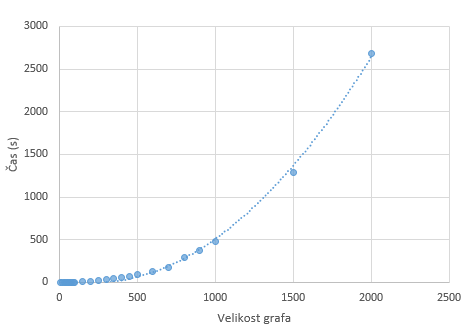
\includegraphics[width=12cm]{casovna_p1_n.png}
  \caption{Časovna zahtevnost pri P1 glede na $n$}
  \label{fig:p1_časovna_zaht_n} 
\end{figure}


\vspace{1cm}

Pri fiksnem številu vozlišč na 100 pa je časovna odvisnost glede na kmax linearna:

\begin{figure}[H]
\centering
  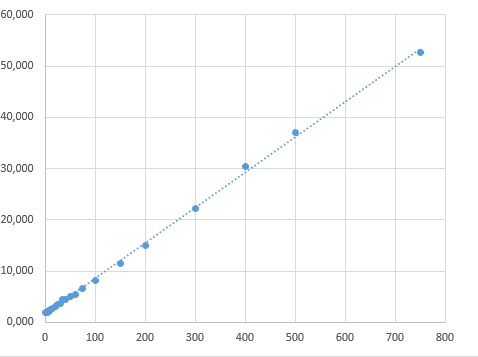
\includegraphics[width=12cm]{casovna_p1_kmax.png}
  \caption{Časovna zahtevnost pri P1 glede na kmax}
  \label{fig:p1_časovna_zaht_kmax} 
\end{figure}

\vspace{1cm}


\subsection{Rezultati in povzetek}

Meniva, da sva našla globalni minimum za poljubno število vozlišč, da je enak 2 in je dosežen pri zvezdah. Našla pa sva še en minimum za soda števila vozlišč n, sestavljen iz dveh zvezd velikosti n/2, povezanih s središčema. Kar se tiče maksimumov, jih je sodeč po točnih rešitvah na manjših grafih in uspešnostjo algoritmov na večjih precej veliko in so običajno po velikosti malo pod številom vozlišč ter največ enaki. Njihovo obliko si lahko ogledamo v shranjenih slikah, vidimo pa, da imajo relativno velik premer.

\pagebreak

\section{Problem P2}

\subsection{Reševanje}

\normalfont{Za manjše grafe, kjer je možno eksaktno računanje, sva napisala funkcijo za generiranje vseh izomorfnih dreves na $n$ vozliščih ter funkcije, ki najprej iz vseh poberejo tista z iskano lastnostjo, to je spremembo Wienerjevega indeksa za 1 ob odstranitvi ene in dodajanju nove povezave kot v opisu problema, nato pa izmed teh vrnejo tisto drevo z največjim premerom, če tako sploh obstaja. To je točna rešitev problema, a je časovno zahtevna ne le generacija grafov, temveč tudi računanje premera. Zato sva za večje $n$ tudi tukaj napisala novo kodo.

Primera dveh dreves, ki sva jih dobila z eksaktnim računanjem.}

\begin{figure}[H]
\centering
  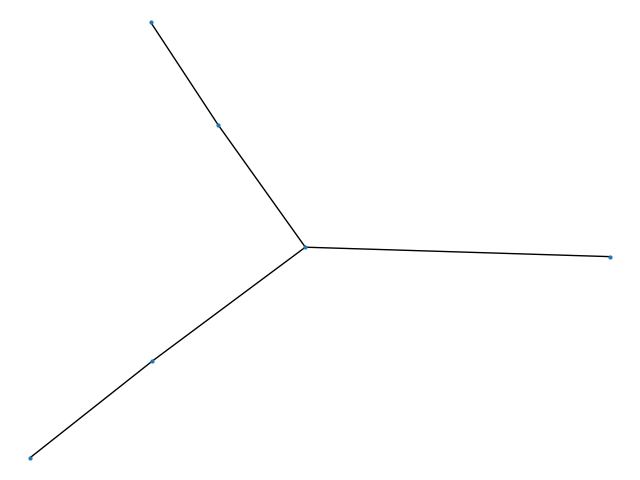
\includegraphics[width=7cm]{drevo6diam4.png}
  \caption{Primer točne rešitve za $n$ = 6, premer = 6}
  \label{fig:graf1} 
\end{figure}

\begin{figure}[H]
\centering
  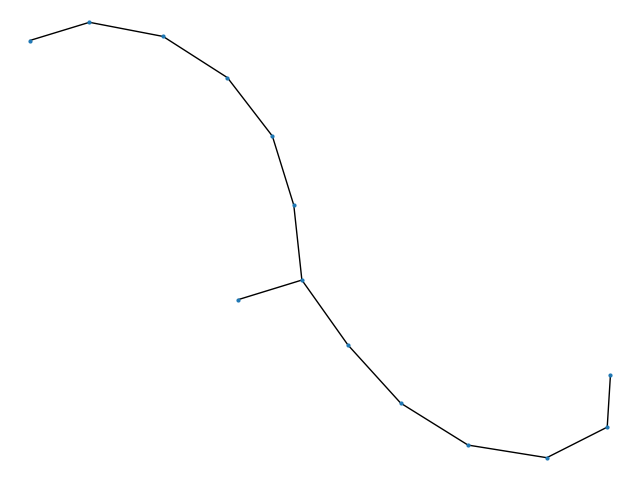
\includegraphics[width=7cm]{drevo14diam12.png}
  \caption{Primer točne rešitve za $n$ = 14, premer = 12}
  \label{fig:graf1}
\end{figure}

\vspace{1cm}

Ideja algoritma za iskanje drevesa na večjem številu vozlišč pri P2 je, da začneva na poti z željenim številom vozlišč in za njo posebej izračunava wienerjev indeks na časovno preprost način. Nato na vsakem koraku odstraniva povezavo iz lista in dodava novo ter glede na prejšnji graf izračunava nov indeks ter ju primerjava, nato pa star graf nadomestiva z novim. To omogoča preverjanje velikega števila grafov, kar je za problem P2 ključno.

Časovna zahtevnost pri spreminjajočem se številu vozlišč $n$ pri 1.000.000 korakih:

\begin{figure}[H]
\centering
  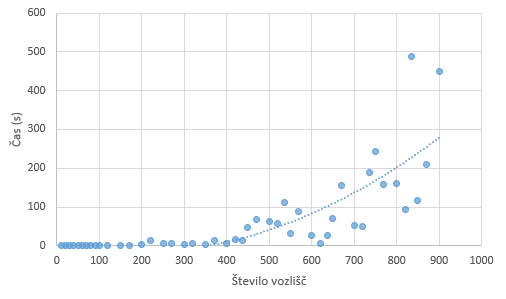
\includegraphics[width=12cm]{casovna_p2_n.png}
  \caption{Časovna zahtevnost pri P2 glede na $n$}
  \label{fig:p2_časovna_zaht_n} 
\end{figure}

\vspace{1cm}

Še časovna zahtevnost pri fiksnem $n = 200$ in različnem številu korakov ohlajanja:

\begin{figure}[H]
\centering
  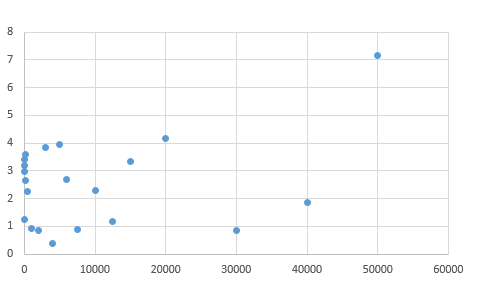
\includegraphics[width=12cm]{casovna_p2_korak.png}
  \caption{Časovna zahtevnost pri P2 glede na število korakov ohlajanja}
  \label{fig:p2_časovna_zaht_korak} 
\end{figure}


\subsection{Rezultati in povzetek}

Očitno je dobrih dreves precej malo, vsekakor dosti manj kot pri P1, saj je treba izvesti ogromno število korakov spreminjanja, da najdemo vsaj eno; to pa še narašča s številom vozlišč; pri 2000 namreč morda celo 1 000 000 ni dovolj. Videti je, da najin algoritem dobiva maksimume v velikosti okoli treh četrtin števila vozlišč. Težko je oceniti kvaliteto rešitev s pomočjo točnih rešitev manjših grafov, saj je koda tako časovno zahtevna, da imava rezultate le to dreves s številom vozlišč 14. Opazila sva tudi, da ne moreva dobiti iskanega drevesa za liho število vozlišč, in to ne le s poskušanjem, ampak tudi na malih grafih. Predpostavljava, da ne obstaja.

\section{Zaključek}


\end{document}